\documentclass[a4paper]{article}

%use the english line for english reports
%usepackage[english]{babel}
\usepackage[english]{babel}
\usepackage[utf8]{inputenc}
\usepackage{indentfirst}
\usepackage{graphicx}
\usepackage{verbatim}
%\usepackage{tabular}
\usepackage[hidelinks]{hyperref}

\begin{document}

\setlength{\textwidth}{16cm}
\setlength{\textheight}{22cm}

\title{\Huge\textbf {Distributed Backup Service} \linebreak\linebreak\linebreak
\Large\textbf {Final Report} \linebreak\linebreak

\includegraphics [height=6cm, width=7cm] {feup.pdf} \linebreak \linebreak
\Large {Master in Informatics and Computing Engineering} \linebreak \linebreak
\Large {Distributed Systems} \linebreak
}

\author{\textbf {Authors:}\\ \centerline {Duarte Nuno Pereira Duarte - 201109179} \\ \centerline  {Ruben Fernando Pinto Cordeiro - 201109177} \\\linebreak\linebreak \\
 \\ Faculdade de Engenharia da Universidade do Porto 
 \\ Rua Roberto Frias, s\/n, 4200-465 Porto, Portugal \linebreak\linebreak\linebreak
\linebreak\linebreak\vspace{1cm}}
%\date{Junho de 2007}
\maketitle
\thispagestyle {empty}

%************************************************************************************************
%************************************************************************************************

\newpage

\tableofcontents

\newpage

\section{Architectural design}

In order to ensure a proficient multi-threaded implementation of the sub protocols, several features of the \textit{.NET Rx} framework were used.

Each one of the \textit{Multicast} channels (MC, MDB and MDR) are modeled as both a MulticastListener and a MulticastBroadcaster class.

The MulticastBroadcaster class encapsulates a socket in order to send data to the network.

The MulticastListener class encapsulates a socket in order to receive data from the network. It also contains a reference to a \textit{System.Reactive.Subject} object. This \textit{Subject} is a provider of asynchronous push-based notifications: for each message received from the socket, all of the \textit{Observers} subscribed to this channel are notified of it's arrival. See figure~\ref{fig:sockets} for more details:

\begin{figure}[h!]
\begin{center}
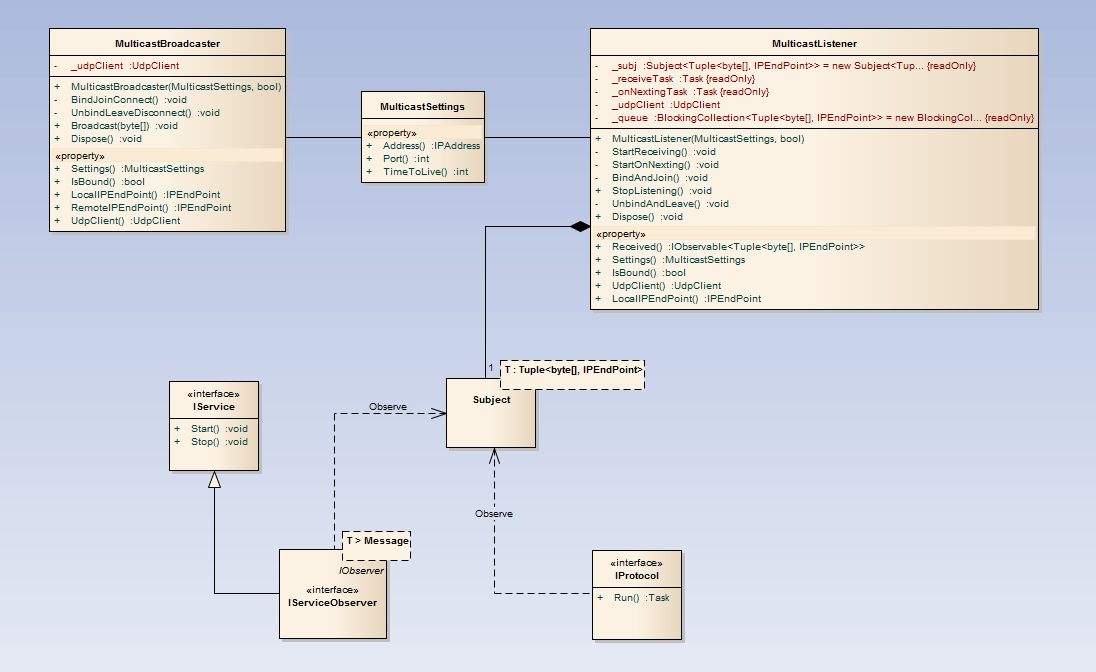
\includegraphics[height=7cm, width=12cm]{figures/socketsUML.PNG}
\caption{Channel UML diagram}
\label{fig:sockets}
\end{center}
\end{figure}

Each one of the sub protocols described in the specification document is modeled as an \textbf{IProtocol} interface. This interface exposes a single method: \textit{Run()}, that initiates an asynchronous System.Threading.Tasks.Task, containing the sequence of all the operations required for the protocol. Several instances of these protocols may be initiated by the peer in a concurrent fashion. See the UML diagram in figure~\ref{fig:protocols}:

\begin{figure}[h!]
\begin{center}
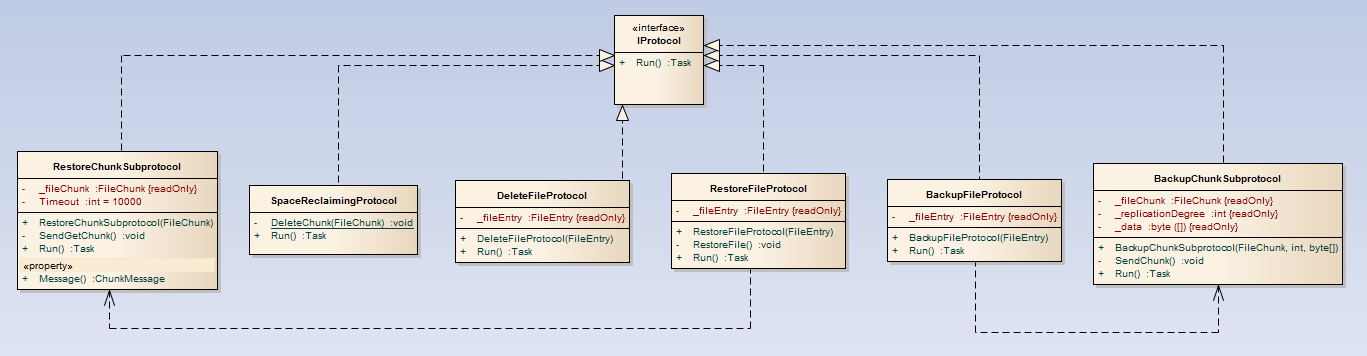
\includegraphics[height=3cm, width=12cm]{figures/protocolsUML.PNG}
\caption{Protocols UML diagram}
\label{fig:protocols}
\end{center}
\end{figure}

Additionally, each one of the \textbf{IProtocol} instances may subscribe to the multicast channels in order to receive message notifications.

Besides explicitly initiating sub protocols, the backup service also provides a set of background services that reply to requests coming from the network. These background tasks are modeled as \textbf{IService} class instances. These services are subscribed to one or more multicast channels, thus receiving asynchronous push-based notifications. See figure~\ref{fig:services} for more details:

\begin{figure}[h!]
\begin{center}
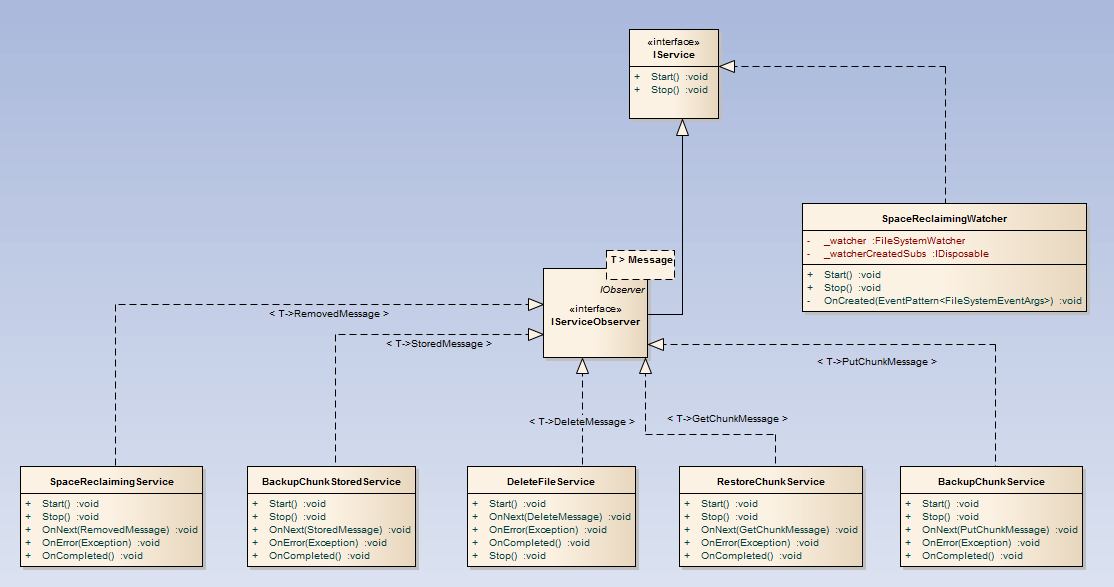
\includegraphics[height=5cm, width=12cm]{figures/servicesUML.PNG}
\caption{Services UML diagram}
\label{fig:services}
\end{center}
\end{figure}

Finally, each message type sent/received through the network is modeled as a \textbf{Message} class. See figure~\ref{fig:messages}:

\begin{figure}[h!]
\begin{center}
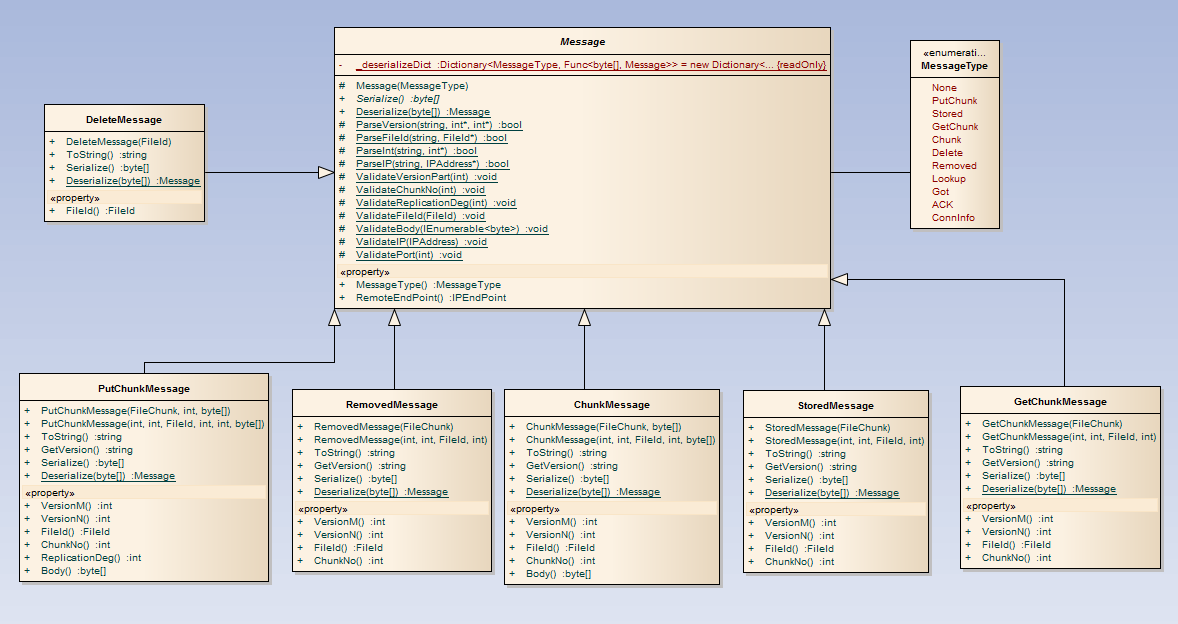
\includegraphics[height=7cm, width=12cm]{figures/messageUML.PNG}
\caption{Messages UML diagram}
\label{fig:messages}
\end{center}
\end{figure}

%************************************************************************
%************************************************************************

\newpage

\section{Enhancements}

All of the enhancements were implemented, the following sections describe the detailed implementation of each enhancement.

\subsection{Data persistence}

The information relative to the replication degree of each backed up chunk is stored in a \textbf{sqlite} database. This ensures constant data persistence. Besides the desired replication degree, the IP address of all the peers that backed up each chunk are also stored. These IP addresses ensure that duplicated \textbf{STORED} messages are not taken into account by each peer. This will be crucial to the enhancements described in section~\ref{sec:backup}.

This database also stores the information about the files backed up by the peer.

%************************************************************************
%************************************************************************
\newpage

\subsection{Chunk backup subprotocol}
\label{sec:backup}

Upon receiving the PUTCHUNK message, each peer checks it's local count of confirmation messages for the specified chunk after the random delay. If the count matches or exceeds the desired replication degree of the chunk, then the peer does not back up the chunk and doesn't reply with a confirmation message.

This optimization avoids the fast depletion of the backup space, since all the peers in the network stop backing up chunks with an actual replication degree higher than the desired.

\subsection{Chunk restore protocol}
\label{sec:restore}

In this enhancement, a peer sends the chunk via a TCP connection instead of sending it in a body of a CHUNK message via the MDR channel.

This new protocol is described in figure~\ref{fig:restoreProtocol}:
\begin{figure}[h!]
\begin{center}
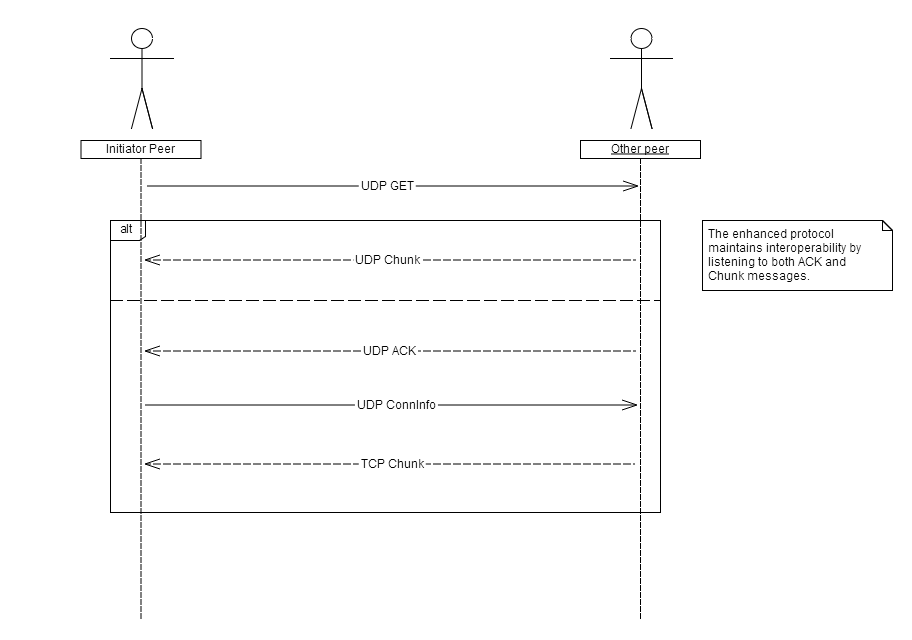
\includegraphics[height=10cm, width=12cm]{figures/enhanced_restore_protocol.png}
\caption{Enhanced restore chunk protocol sequence diagram}
\label{fig:restoreProtocol}
\end{center}
\end{figure}

For this purpose, two new message types were added: \textbf{ACK} and \textbf{CONNINFO} messages. These messages have the following structure:

\begin{verbatim}
ACK <Version> <FileId> <ChunkNo> <CRLF> <CRLF>

CONNINFO <Version> <FileId> <ChunkNo> <InitiatorPeerPort>
<SelectedPeerIP> <CRLF> <CRLF>
\end{verbatim}

\begin{description}
\item[InitiatorPeerPort]: selected TCP port by the initiator peer.
\item[SelectedPeerIP]: IP address of the peer that has sent the first ACK message.
\end{description}

The initiator peer sends a GETCHUNK message via the MC channel. After that, the initiator peer waits for either a CHUNK or ACK message. If the CHUNK message is the first to arrive, the protocol finishes, otherwise, a CONNINFO message is sent via the MC channel. The initiator peer opens the TCP connection and waits for the other peer to open it as well. This ensures the protocol interoperability: we are still able to restore data from non conforming peers.

Upon receiving a GETCHUNK message, a peer with the requested chunk sends an ACK message after a random delay uniformly distributed between 0 and 400 ms.
Only the peer with the IP address equal to the \textbf{SelectedPeerIP} field of the CONNINFO message actually opens the TCP connection and sends the requested chunk, every other peer discards it.

By setting up a TCP connection, we're sending chunks in a more reliable channel while reducing the load on the MC and MDR channels.
%************************************************************************
%************************************************************************
\newpage

\subsection{File deletion subprotocol}

In order to reclaim space occupied by unused chunks, each peer periodically initiates a \textbf{Lookup} protocol.

This protocol consists in the following operations:

\begin{itemize}
	\item Initiator peer:
		\begin{enumerate}
			\item Create a list with all the distinct fileId's associated with every backed up chunk.
			\item Send a LOOKUP message for each distinct fileId via the MC channel and listen for GOT messages during a timeout interval (starts at 1 second).
			\item Repeat step 2 up to 5 times, doubling the timeout interval in each iteration.
			\item Delete all the backed up chunks associated to a fileId that wasn't acknowledged via a GOT message.
		\end{enumerate}
		
	\item Other peers:
		\begin{enumerate}
			\item For every LOOKUP message received, check if the fileId corresponds to a backed up file. If it does, reply with a GOT message for the same fileId.
		\end{enumerate}
\end{itemize}

The LOOKUP and GOT messages have the following structure:

\begin{verbatim}
LOOKUP <Version> <FileId> <CRLF> <CRLF>
GOT <Version> <FileId> <CRLF> <CRLF>
\end{verbatim}

This protocol ensures that only chunks belonging to active peers in the network are backed up.
%************************************************************************
%************************************************************************

\subsection{Space reclaiming subprotocol}

In order to tolerate chunk backup subprotocol failures and increase the replication degree of each chunk to the desired value, a new background service was implemented: \textbf{EnhancedSpaceReclaimingWatcher}. This service runs periodically and contemplates the following operations:

\begin{enumerate}
	\item Initiate a chunk backup subprotocol for every chunk with an actual replication degree lower than the desired. Give priority to the chunks with the biggest replication degree offset.
	\item Remove all the chunks with an actual replication degree higher than the desired.
\end{enumerate}

Besides this new service, a new enhancement was introduced in the restore chunk protocol: upon receiving a GETCHUNK message, check the the database for the chunk entry. If there's an entry in the database but the actual chunk is missing in the backup directory, send a REMOVED message with the given fileId and chunkNo and remove the entry from the database, since the peer in question was supposed to have a local backup of the chunk. This enhancement tolerates faults from the local filesystem or external interference (chunk erased outside the program).

%************************************************************************
%************************************************************************

 \end{document}
